\documentclass[10pt,a4paper]{article}
\usepackage[margin=20mm]{geometry}
\usepackage[T1]{fontenc}
\usepackage[utf8]{inputenc}
\usepackage{lmodern,amsmath,amssymb,booktabs,longtable,array,graphicx,xurl,fvextra}
\usepackage[hidelinks]{hyperref}
\RecustomVerbatimEnvironment{verbatim}{Verbatim}{breaklines=true,breakanywhere=true,fontsize=\scriptsize}
\setlength{\parindent}{0pt}\setlength{\parskip}{5pt}
\title{A011 --- Maxwell SST Kinetic Falsifier\\v0.4.1 Scientific Protocol and Falsifier Report}
\author{SST-Workbench}
\date{Framework v1.0.10; controlled geometry diagnostic tranche}
\begin{document}\maketitle
% SST-REPORT-SECTION:IDENTIFICATION
\section{Identification, version and authority}
A011 v0.4.1 is a packaging/report binding patch of the preserved v0.4.0 geometry pilot. It uses the byte-qualified SST Falsifier Framework v1.0.10. Equations, source geometry, parity thresholds and physical input requirements are unchanged. Scientific claims remain unresolved; software execution is not physical certification.
% SST-REPORT-SECTION:QUESTION
\section{Research question and scientific objective}
Does the v1.0.10 adapter retain inherited A011 geometry definitions and Python/native consistency on exact admitted PKLSA inputs?

Qualify software migration and bounded geometry diagnostics while explicitly withholding physical closure.
% SST-REPORT-SECTION:HYPOTHESES
\section{Null and alternative hypotheses; falsification criteria}
\paragraph{$H_0$.} Adapter source admission or the inherited native/reference tolerances fail on the preregistered geometry set.\paragraph{$H_1$.} Exact admitted geometry is processed with finite inherited diagnostics and existing native/reference tolerances; no physical prediction follows.
\begin{itemize}
\item F1: Any source hash/capability mismatch aborts execution; no substitution. Recorded consequence: FAIL\_INFRASTRUCTURE
\item F2: Native parity outside original tolerances is a failed implementation smoke. Recorded consequence: FAIL
\item F3: Unavailable independent physical inputs cannot support physical discovery or closure. Recorded consequence: NOT\_RUN\_PREREQUISITE
\end{itemize}
% SST-REPORT-SECTION:ASSUMPTIONS
\section{Assumptions, domain and edge cases}
\begin{enumerate}\item Input coordinate units are source-native and have no certified SI scale.
\item Closed polygon curves are resampled by the unchanged A011 reference definition.
\item Two resolutions expose sensitivity only.
\item No energy spectrum, gravity or thermodynamic state-count evidence is inferred from curves.\end{enumerate}
Registered edge cases: Missing native ABI-compatible binary; Raw/geometry hash drift; Nonfinite or degenerate geometry; Existing output directory; No calibrated SI scale
% SST-REPORT-SECTION:SYMBOLS
\section{Symbols, definitions, SI units and dimensional audit}
\begin{longtable}{p{0.11\linewidth}p{0.31\linewidth}p{0.29\linewidth}p{0.18\linewidth}}\toprule Symbol & Definition & SI unit / scale & Dimensions\\\midrule
$p_i$ & Source-native polygon vertex & Uncalibrated source coordinate unit & L in a declared native unit \\
$L$ & Resampled polygon length & Uncalibrated source coordinate unit & L \\
$Wr$ & Inherited midpoint writhe diagnostic & 1 & 1 \\
\bottomrule\end{longtable}
$v_{cpp,j}$ and $v_{py,j}$ are the corresponding native/reference kernel-test components in E2; $N$ counts resampled points. Curvature has inverse native-coordinate units. There is no independently calibrated SI length/time conversion. Gamma=1, smoothing=0.05 and the fixed probe offset are nondimensional software probes, not measured physical inputs.
% SST-REPORT-SECTION:EQUATIONS
\section{Registered equations and code-to-mathematics mapping}
% AUTO-GENERATED. Do not edit; generated from frozen science_contract.json.
\subsection*{Machine-readable science contract}
\begin{description}
\item[Research question] Does the v1.0.10 adapter retain inherited A011 geometry definitions and Python/native consistency on exact admitted PKLSA inputs?
\item[Objective] Qualify software migration and bounded geometry diagnostics while explicitly withholding physical closure.
\item[$H_0$] Adapter source admission or the inherited native/reference tolerances fail on the preregistered geometry set.
\item[$H_1$] Exact admitted geometry is processed with finite inherited diagnostics and existing native/reference tolerances; no physical prediction follows.
\end{description}
\subsubsection*{Registered equations}
\paragraph{E1: Inherited polygon length}
\begin{equation}
L=\sum_i\|p_{i+1}-p_i\|
\end{equation}
\noindent\textit{Dimensional check:} Coordinate length; no SI conversion without calibration.\\
\paragraph{E2: Existing componentwise velocity parity criterion}
\begin{equation}
|v_{cpp,j}-v_{py,j}|\le 10^{-12}+10^{-11}|v_{py,j}|
\end{equation}
\noindent\textit{Dimensional check:} Same nondimensional test-kernel convention on both implementations; no physical velocity claim.\\
\subsubsection*{Registered code-to-mathematics steps}
\begin{enumerate}
\item \textbf{S1} [G1; equations E1]: Rehash qualified source, protocol, exact admitted raw and parsed geometry inputs
\item \textbf{S2} [G2; equations E1]: Apply unchanged A011 resampling and geometry definitions
\item \textbf{S3} [G5; equations E2]: Compare inherited native and transparent reference kernels despite missing physical prerequisites
\end{enumerate}

Only the equations registered in the inherited science contract are asserted here. Other inherited geometry diagnostics are defined by the cited implementation; no missing physical model is invented.
% SST-REPORT-SECTION:ALGORITHM
\section{Algorithm, phases and execution order}
\begin{enumerate}\item Verify qualified framework, frozen geometry protocol and report/output binding.\item Run targeted tests before any fresh bounded smoke.\item Rehash the three admitted carrier descriptors, source bytes, parsed geometry and qualification evidence.\item Apply the unchanged A011 resampling and geometry kernels at N=64 and N=128.\item Attempt independent implemented evaluators despite unavailable physical prerequisites; record raw outcomes and recursive qualification separately.\item Seal machine evidence; generate scientific TeX with the existing framework; compile the PDF; publish a unique ZIP and SHA-256 sidecar.\end{enumerate}
% SST-REPORT-SECTION:SOURCES
\section{Sources, provenance and dataset qualification}
Only the exact sources in source\_contract.json and the Phase 2 A011 admission ledger are used. Raw and parsed geometry hashes and prerequisite capability records are reverified. All three are numerical KnotPlot geometry sources, not independent physical replications. The complete current source manifest is included by the automatic results section. The qualified framework and E010 parser pins remain separate from scientific qualification.
% SST-REPORT-SECTION:GATES
\section{Migration, execution and scientific gates}
Migration, execution and scientific statuses are separate axes. G0/G1 verify protocol/source integrity; G2 measures finite geometry diagnostics. G5 measures actual native/reference parity but remains DIAGNOSTIC\_ONLY when G3/G4 physical prerequisites are unavailable. G3/G4/G7/G8 remain not executed for missing evidence. GPU G6 is disabled and reveal G9 is deferred. Exact current records, qualifications and allows-dependent-claim fields are generated directly from the machine ledger below.
% SST-REPORT-SECTION:NUMERICS
\section{Numerical methods, tolerances and convergence criteria}
Unchanged uniform polygon arclength resampling, discrete geometry diagnostics and FP64 kernels from A011 v0.3.1 are used. The frozen ladder is $N=64,128$. Native/reference velocity uses rtol=$10^{-11}$ and atol=$10^{-12}$; writhe and distance require absolute deltas $<10^{-11}$. No NaN/Inf, source drift or missing native module is replaced by a warning. These two resolutions expose sensitivity only: no spatial, time, solver or regularization convergence certificate is claimed. Missing physical error budgets remain unresolved.
% SST-REPORT-SECTION:BACKENDS
\section{Backend manifest and authority}
CPython 3.14/NumPy FP64 is the transparent reference. The inherited byte-pinned Windows cp314 C++17 kernel is used without rebuilding or silent fallback; its legacy backend version remains 0.3.1-cpp17. This is geometry-kernel implementation evidence only. No GPU, physical solver parity or independently authenticated compiler rebuild is claimed. Actual environment and binary/source hashes are rendered below.
% SST-REPORT-SECTION:BLINDNESS
\section{Blind/reveal boundaries}
No private target is opened, no expected winner is optimized and no reveal is performed. This is a nonrevealed geometry-diagnostic adapter run, not the complete private-target BLIND/REVEAL experiment. The generic framework automatic provenance uses BLIND for unrevealed output; in this report that label does not assert a completed physical blind campaign. No historical dataset seal or blind/reveal commitment is modified.
% SST-REPORT-SECTION:STATISTICS
\section{Uncertainty, independence and statistical limits}
The three representative topologies are fixed in advance; carrier ordering is lexicographic after exact admission and size filters. There is no random sample, fitted parameter, p-value or population-level significance claim. The common source lineage does not provide independent replication. Resolution differences, parity residuals and missing physical uncertainty are reported separately.
% SST-REPORT-SECTION:RESULTS
\section{Automatic results, tables and diagnostic graphs}
\subsection*{Separate migration, execution and scientific axes}
\begin{longtable}{p{0.25\linewidth}p{0.68\linewidth}}\toprule Axis & Actual status\\\midrule
migration\_\allowbreak{}gate & PASS\_\allowbreak{}GEOMETRY\_\allowbreak{}ADAPTER \\
execution\_\allowbreak{}gate & PASS\_\allowbreak{}BOUNDED\_\allowbreak{}GEOMETRY\_\allowbreak{}SMOKE \\
scientific\_\allowbreak{}gate & UNRESOLVED\_\allowbreak{}MISSING\_\allowbreak{}PHYSICAL\_\allowbreak{}INPUTS \\
scientific\_\allowbreak{}status\_\allowbreak{}promoted & False \\
\bottomrule\end{longtable}
\subsection*{Measured geometry and resolution sensitivity}
\begin{longtable}{p{0.15\linewidth}rrrr}\toprule Topology & N & Native length & Mean curvature & Midpoint writhe\\\midrule
0\_1 & 64 & 12.52869104 & 0.5033844161 & 0 \\
0\_1 & 128 & 12.54017859 & 0.6604430041 & 0 \\
3\_1 & 64 & 16.32543462 & 0.9829584087 & 3.412398906 \\
3\_1 & 128 & 16.36257488 & 1.034079532 & 3.408273635 \\
4\_1 & 64 & 22.35286777 & 0.910604241 & 0.2068828022 \\
4\_1 & 128 & 22.44280283 & 0.9558892656 & 0.2007498053 \\
\bottomrule\end{longtable}
Two registered levels expose sensitivity; they do not establish convergence or physical calibration.
\begin{figure}[htbp]\centering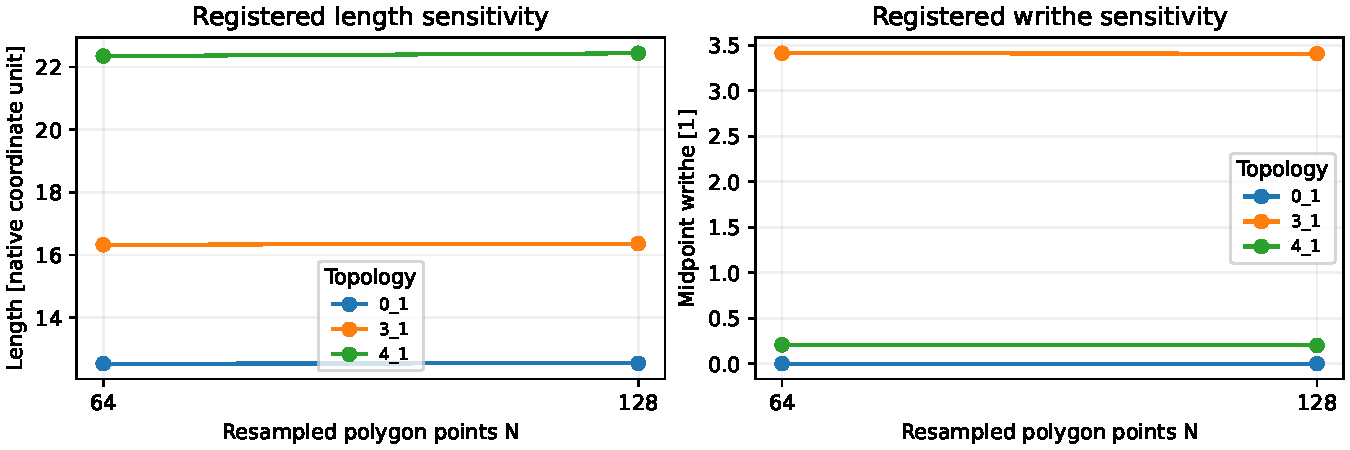
\includegraphics[width=\linewidth]{figures/geometry_sensitivity.pdf}\caption{Actual N=64 and N=128 measurements from PLOT\_DATA.json. Native lengths have no calibrated SI scale; writhe is dimensionless. No fitted trend or continuum extrapolation.}\end{figure}
\subsection*{Actual native/reference comparisons}
\begin{longtable}{p{0.15\linewidth}rrrr}\toprule Carrier topology & N & Velocity max abs & Writhe abs & Distance abs\\\midrule
0\_1 & 64 & 2.7756e-17 & 0 & 0 \\
0\_1 & 128 & 6.9389e-18 & 0 & 0 \\
3\_1 & 64 & 5.5511e-17 & 0 & 0 \\
3\_1 & 128 & 5.5511e-17 & 0 & 0 \\
4\_1 & 64 & 2.2204e-16 & 0 & 0 \\
4\_1 & 128 & 2.2204e-16 & 0 & 0 \\
\bottomrule\end{longtable}
\subsection*{Exact gate execution and claim authority}
\begin{longtable}{p{0.08\linewidth}p{0.28\linewidth}p{0.34\linewidth}p{0.19\linewidth}}\toprule Gate & Execution & Qualification & Allows dependent claim\\\midrule
G0 & EXECUTED & QUALIFIED & True \\
G1 & EXECUTED & QUALIFIED & True \\
G2 & EXECUTED & QUALIFIED & True \\
G3 & NOT\_\allowbreak{}EXECUTED & BLOCKED\_\allowbreak{}PREREQUISITE & False \\
G4 & NOT\_\allowbreak{}EXECUTED & BLOCKED\_\allowbreak{}PREREQUISITE & False \\
G5 & EXECUTED & DIAGNOSTIC\_\allowbreak{}ONLY & False \\
G6 & DISABLED & NOT\_\allowbreak{}APPLICABLE & False \\
G7 & NOT\_\allowbreak{}EXECUTED & BLOCKED\_\allowbreak{}PREREQUISITE & False \\
G8 & NOT\_\allowbreak{}EXECUTED & BLOCKED\_\allowbreak{}PREREQUISITE & False \\
G9 & DEFERRED & DEFERRED & False \\
\bottomrule\end{longtable}
\subsection*{Missing scientific evidence}
\begin{itemize}
\item Calibrated physical length and SI source scale
\item Independent physical energy spectrum/gaps and relaxation/couplings
\item Independent thermodynamic sampled state counts
\item Held-out force/pressure and mechanism validation
\item Spatial/time/solver/regularization convergence beyond this two-level geometry smoke
\end{itemize}
% AUTO-GENERATED. Do not edit.
\subsection*{Automatic run provenance}
\begin{longtable}{p{0.28\linewidth}p{0.64\linewidth}}
\toprule
Field & Recorded value \\
\midrule
Run ID & 20261026T183440820118Z-\allowbreak{}6ec84069 \\
Run phase & BLIND \\
Protocol bundle SHA-256 (byte exact) & 4f599c7dd917\allowbreak{}844ca2d43227\allowbreak{}0b4b0a607c2d\allowbreak{}0a6ccf3d9eaf\allowbreak{}6243a1224a8a\allowbreak{}44bf \\
Portable protocol diagnostic SHA-256 & c64f3320dbe3\allowbreak{}cfac0fe3a70a\allowbreak{}e2ffc5f3adf8\allowbreak{}6675e11d1f43\allowbreak{}871c767eb3ff\allowbreak{}ba98 \\
Framework schema & SST-\allowbreak{}FALSIFIER-\allowbreak{}PROTOCOL-\allowbreak{}2 \\
Python & 3.14.3 (tags/\allowbreak{}v3.14.3:323c59a, Feb  3 2026, 16:04:56) [MSC v.1944 64 bit (AMD64)] \\
Platform & Windows-\allowbreak{}11-\allowbreak{}10.0.26300-\allowbreak{}SP0 \\
Science evidence SHA-256 & 0c3802ccee9f\allowbreak{}974da0b6240d\allowbreak{}c61545ca6fa5\allowbreak{}0a66a4a824c2\allowbreak{}17e381f1b35e\allowbreak{}191b \\
Final output manifest & See OUTPUT\_\allowbreak{}MANIFEST.json (finalized after PDF and report metadata) \\
\bottomrule
\end{longtable}
\subsubsection*{Gate ledger}
\begingroup\small\setlength{\tabcolsep}{3pt}\begin{longtable}{p{0.07\linewidth}p{0.19\linewidth}p{0.31\linewidth}p{0.29\linewidth}}
\toprule
Gate & Status & Question & Reason \\
\midrule
{\ttfamily\scriptsize G0} & {\ttfamily\footnotesize PASS} & Are the qualified framework and dedicated adapter protocol byte-\allowbreak{}exact? & Qualified framework and dedicated adapter protocol verified; not the full framework blind/\allowbreak{}reveal FREEZE. \\
{\ttfamily\scriptsize G1} & {\ttfamily\footnotesize PASS} & Do all selected geometry sources satisfy exact admission and hashes? & Rehashed exact admitted geometry and prior capability evidence; geometry authority only. \\
{\ttfamily\scriptsize G2} & {\ttfamily\footnotesize PASS} & Are inherited geometry metrics finite under the fixed bounded ladder? & Inherited geometry definitions, native units and registered smoke budget; no physical closure. \\
{\ttfamily\scriptsize G3} & {\ttfamily\footnotesize NOT\_\allowbreak{}RUN\_\allowbreak{}PREREQUISITE} & Are independent physical discovery inputs available and qualified? & Required scientific inputs unavailable: Independent physical energies, gaps, relaxation/\allowbreak{}couplings, sampled state counts, force/\allowbreak{}pressure holdouts and calibrated SI scale are not supplied by the admitted geometry atlas. \\
{\ttfamily\scriptsize G4} & {\ttfamily\footnotesize NOT\_\allowbreak{}RUN\_\allowbreak{}PREREQUISITE} & Does independent physical held-\allowbreak{}out evidence confirm a mechanism? & Required scientific inputs unavailable: Independent physical energies, gaps, relaxation/\allowbreak{}couplings, sampled state counts, force/\allowbreak{}pressure holdouts and calibrated SI scale are not supplied by the admitted geometry atlas. \\
{\ttfamily\scriptsize G5} & {\ttfamily\footnotesize PASS} & Does the inherited native geometry kernel match reference tolerances? & Measured despite unavailable physical prerequisites; parity never certifies physical SST. \\
{\ttfamily\scriptsize G6} & {\ttfamily\footnotesize NOT\_\allowbreak{}APPLICABLE} & GPU screening (disabled in this CPU geometry tranche) & Disabled by framework profile \\
{\ttfamily\scriptsize G7} & {\ttfamily\footnotesize NOT\_\allowbreak{}RUN\_\allowbreak{}PREREQUISITE} & Is independent physical replication available? & Required scientific inputs unavailable: Independent physical energies, gaps, relaxation/\allowbreak{}couplings, sampled state counts, force/\allowbreak{}pressure holdouts and calibrated SI scale are not supplied by the admitted geometry atlas. \\
{\ttfamily\scriptsize G8} & {\ttfamily\footnotesize NOT\_\allowbreak{}RUN\_\allowbreak{}PREREQUISITE} & Is physical mechanism and convergence evidence available? & Required scientific inputs unavailable: Independent physical energies, gaps, relaxation/\allowbreak{}couplings, sampled state counts, force/\allowbreak{}pressure holdouts and calibrated SI scale are not supplied by the admitted geometry atlas. \\
{\ttfamily\scriptsize G9} & {\ttfamily\footnotesize DEFERRED} & Reveal is separate and not allowed in this geometry-\allowbreak{}only tranche & No reveal requested or permitted by this geometry-\allowbreak{}only tranche. \\
\bottomrule
\end{longtable}\endgroup
\subsubsection*{Scientific qualification (separate from measured gate outcomes)}
\begingroup\small\setlength{\tabcolsep}{3pt}\begin{longtable}{p{0.13\linewidth}p{0.37\linewidth}p{0.38\linewidth}}
\toprule
Gate & Evidence qualification & Blocking prerequisites \\
\midrule
G0 & QUALIFIED & none \\
G1 & QUALIFIED & none \\
G2 & QUALIFIED & none \\
G3 & BLOCKED\_\allowbreak{}PREREQUISITE & none \\
G4 & BLOCKED\_\allowbreak{}PREREQUISITE & G3 \\
G5 & DIAGNOSTIC\_\allowbreak{}ONLY & G4 \\
G6 & NOT\_\allowbreak{}APPLICABLE & G5 \\
G7 & BLOCKED\_\allowbreak{}PREREQUISITE & G6 \\
G8 & BLOCKED\_\allowbreak{}PREREQUISITE & G7 \\
G9 & DEFERRED & G8 \\
\bottomrule
\end{longtable}\endgroup
\subsubsection*{Backend manifest}
\begingroup\footnotesize\begin{verbatim}
{
  "actual_backend": {
    "backend": "cpp",
    "native": true,
    "version": "0.3.1-cpp17"
  },
  "authority": "GEOMETRY_KERNEL_ONLY",
  "gpu_used": false,
  "native_binary_sha256": 
"9c387369427ff986101d4f345ac75d2a24d8ec640f24999132b3fc351f5294f6",
  "native_cpp_sha256": 
"00bd3ae13925fb176b501b676c89e4a95c72b6ac0cea6fd297b0b0b990dcf0cd",
  "native_rebuilt": false,
  "numpy": "2.4.4",
  "physical_qualification": "UNRESOLVED",
  "python": "3.14.3 (tags/v3.14.3:323c59a, Feb  3 2026, 16:04:56) [MSC v.1944
 64 bit (AMD64)]",
  "schema": "SST-BACKEND-MANIFEST-2"
}
\end{verbatim}\endgroup
\subsubsection*{Source manifest}
\begingroup\footnotesize\begin{verbatim}
{
  "manifest_sha256": 
"616420b8dbd5d89777e7bfd9558518b5805a6c91bdb33f64e2019cc718bd516f",
  "schema": "SST-SOURCE-MANIFEST-2",
  "sources": [
    {
      "catalog_id": "E010",
      "evidence_class": "simulation",
      "exists": true,
      "independence_family": "knotplot_relaxation",
      "path": "C:\\workspace\\projects\\SST-Workbench\\03_data\\A_knots\\04_k
notplot\\knot_0.1\\knot_0.1_trial_015k_rr_010k_coarse.rr\\knot_0.1_trial_015k
_rr_010k_coarse.atstart.vect",
      "provenance_family": null,
      "registry_hint": {
        "catalog_id": "E010",
        "hits": []
      },
      "role": "admitted_geometry_diagnostic",
      "sha256": 
"54d6e30010753bb15e4a47f84ec874a0420bcd3bc5e5264edd1a54b508467c3f",
      "source_id": "CAR_17fca17caa5ca443",
      "version": "E010-v0.3.1/view-v0.3.4"
    },
    {
      "catalog_id": "E010",
      "evidence_class": "simulation",
      "exists": true,
      "independence_family": "knotplot_relaxation",
      "path": "C:\\workspace\\projects\\SST-Workbench\\03_data\\A_knots\\04_k
notplot\\knot_3.1\\knot_3.1_trial_002k_rr_010k_coarse_rr_050k_eqfinal_rr_030k
_polish.vect",
      "provenance_family": null,
      "registry_hint": {
        "catalog_id": "E010",
        "hits": []
      },
      "role": "admitted_geometry_diagnostic",
      "sha256": 
"1ef9ced21943e4d87addf3a2988e29b0eaf5afbdab334641a469049605a743ef",
      "source_id": "CAR_042c4a4f554aef25",
      "version": "E010-v0.3.1/view-v0.3.4"
    },
    {
      "catalog_id": "E010",
      "evidence_class": "simulation",
      "exists": true,
      "independence_family": "knotplot_relaxation",
      "path": "C:\\workspace\\projects\\SST-Workbench\\03_data\\A_knots\\04_k
notplot\\knot_4.1\\knot_4.1_trial_001k_rr_010k_coarse_rr_050k_eqfinal.rr\\kno
t_4.1_trial_001k_rr_010k_coarse_rr_050k_eqfinal.vect",
      "provenance_family": null,
      "registry_hint": {
        "catalog_id": "E010",
        "hits": []
      },
      "role": "admitted_geometry_diagnostic",
      "sha256": 
"50b548c10790e94457bfe8e414ba9e7f144ff6b12cea46e63f870eb9d460a333",
      "source_id": "CAR_0b173a215edeb25c",
      "version": "E010-v0.3.1/view-v0.3.4"
    }
  ],
  "workbench_root": "C:\\workspace\\projects\\SST-Workbench"
}
\end{verbatim}\endgroup

% SST-REPORT-SECTION:INTERPRETATION
\section{Interpretation, falsification limits and unresolved claims}
A finite geometry metric or kernel-parity PASS supports only the named implementation diagnostic. It does not establish an energy spectrum, thermodynamic closure, gravity, Euler/Casimir mechanism or new SST prediction. A parity or numerical failure is a failed software check, not independent physical falsification. Missing source calibration, held-out fields, energies, gaps, state counts and convergence evidence remain explicit. Historical negatives and prior runs are preserved.
% SST-REPORT-SECTION:REPRODUCIBILITY
\section{Reproducibility and execution instructions}
From this version directory on Windows execute \texttt{run\_all.cmd}; \texttt{run\_all.cmd SELFTEST} runs tests only. CPython 3.14, the pinned native binary and the qualified local framework/source paths are required. Scientific PDF generation uses the framework LaTeX compiler and fails closed if it cannot compile. Outputs use the declared catalog/family prefix and \texttt{\_outputs}; prior canonical output is retained under its run ID. PDF and ZIP publications are one directory above this version and include immutable run IDs. The adjacent SHA-256 verifies each ZIP. \texttt{LATEST\_RUN.json} is the only replaceable publication pointer; \texttt{PUBLICATIONS.jsonl} is append-only.
\section{References and primary reproducibility records}
\begin{enumerate}
\item \texttt{science\_contract.json}, original registered hypotheses, symbols, equations E1/E2 and code-to-equation steps.
\item \texttt{src/maxwell\_sst\_falsifier/geometry.py}, exact inherited geometric definitions; \texttt{native\_ext/fallback.py} and \texttt{cpp/native.cpp}, reference/native kernels.
\item \texttt{provenance/A011\_DATASET\_ADMISSION.json} and carrier decision ledger; exact E010 parser code pins and raw/geometry source hashes.
\item \texttt{preregistration/FROZEN\_PROTOCOL.json} and \texttt{FRAMEWORK\_SOURCE\_PIN.json}: byte-exact geometry protocol and qualified v1.0.10 source.
\item Current \texttt{GATE\_LEDGER.json}, \texttt{REPORT\_DATA.json}, \texttt{SCIENCE\_EVIDENCE\_MANIFEST.json} and final \texttt{OUTPUT\_MANIFEST.json}.
\end{enumerate}
\end{document}
